\documentclass[11pt, a4paper, lithuanian]{article}

\usepackage[left=25mm,right=15mm,top=15mm,bottom=15mm]{geometry}
\usepackage[utf8x]{inputenc}
\usepackage[L7x]{fontenc}
\usepackage[lithuanian]{babel}
\usepackage{listings}
\usepackage{amsmath, amssymb}
\usepackage{graphicx}

\author{AKSfm-15, Maksim Norkin}
\title{Daugiasluoksnio perceptrono mokymas}

\lstset{
  language=Matlab,
  basicstyle=\footnotesize,
  columns=fixed,
  numbers=none,
  showspaces=false,
  xleftmargin=20pt
}

\begin{document}

    \maketitle

    \section{Užduotis}

    Nenaudodami MATLAB specializuotų funkcijų, sukurkite daugiasluoksnį (dviejų sluoksnių) perceptronų tinklą ir jį apmokykite pasirinktai kreivei (sudarytai iš 20 atskaitų) aproksimuoti. Tinklo apmokymui įgyvendinkite Backpropagation algoritmą. Aktyvavimo funkcijas neuronų tinkle panaudokite savo nuožiūra. Kreive galite sukurti, pavyzdžiui, naudodami kelias trigonometrines funkcijas.

    \section{Pradinės sąlygos}

    Daugiasluoksnį perceptroną pasirinksime dviejų sluoksnių. Pirmas sluoksnis sudarytas iš trijų perceptronų, kurių aktyvavimo funkcija yra eksponentė. Antras sluoksnis, sudarytas iš vieno perceptrono, kurio aktyvavimo funkcija yra tiesinė.

    Pabandysime apkroksimuoti vieną šeštąją periodo, sinuso tipo, signalą.

    \section{Mokymas}

    Mokymas prasideda nuo pradinių įverčių pasirinkimo pirmam sluoksniui ir antram sluoksniui. Įėjimo ir bazės įverčiai pasirenkami, panaudojus \textit{rand} funkcija matlab programiniame pakete. Tokia pačia funkcija yra panaudojama ir antro sluoksnio įėjimo ir bazės įverčiams inicijuoti.

    Toliau yra vykdomas mokymas. Pirmiausiai reikia apskaičiuoti įėjimo sumą pirmam sluoksniui, kiekvienam iš perceptronui, \ref{code:pirmo_sluoksnio_iejimo_funkcijos_apskaiciavimas} pav.

    \begin{figure}[h]
      \centering
      \caption{Pirmo sluoksnio įėjimo sumos apskaičiavimas.}
      \label{code:pirmo_sluoksnio_iejimo_funkcijos_apskaiciavimas}
      \begin{lstlisting}
v1_1 = w1_1 * x + b1_1;
v1_2 = w1_2 * x + b1_2;
v1_3 = w1_3 * x + b1_3;
      \end{lstlisting}
    \end{figure}

    Su pasirinkta eksponentine funkcija kiekvienam iš perceptronų, galima apskaičiuoti išėjimo funkcijos įverčius, \ref{code:pirmo_sluoksnio_funkcijos_apskaiciavimas} pav.

    \begin{figure}[h]
      \centering
      \caption{Pirmo sluoksnio funkcijos apskaičiavimas.}
      \label{code:pirmo_sluoksnio_funkcijos_apskaiciavimas}
      \begin{lstlisting}
y1_1 = 1/(1+exp(-v1_1));
y1_2 = 1/(1+exp(-v1_2));
y1_3 = 1/(1+exp(-v1_3));
      \end{lstlisting}
    \end{figure}

    Apskaičiavus kiekvieno pirmo sluoksnio išėjimo įverčius, toliau galime skaičiuoti antro sluoksnio perceptrono įėjimo sumą ir perdavimo funkciją. Perdavimo funkcija pasirinkta linijinė, todėl atskirai sumos skaičiavimą galima praleisti ir iškarto skaičiuoti perdavimo funkcijos vertę, \ref{code:antro_sluoksnio_funkcijos_apskaiciavimas} pav.

    \begin{figure}[h]
      \centering
      \caption{Antro sluoksnio funkcijos apskaičiavimas.}
      \label{code:antro_sluoksnio_funkcijos_apskaiciavimas}
      \begin{lstlisting}
y2 = y1_1 * w2_1 + y1_2 * w2_2 + y1_3 * w2_3 + b2;
      \end{lstlisting}
    \end{figure}

    Šitame žingsnyje jau turime viso mūsų modelio išėjimo vertę, todėl galima imti ir skaičiuoti viso tinklo momentinė klaidą, \ref{code:modelio_klaidos_skaiciavimas} pav.

    \begin{figure}[h]
      \centering
      \caption{Modelio momentinės klaidos skaičiavimas.}
      \label{code:modelio_klaidos_skaiciavimas}
      \begin{lstlisting}
e2 = y2 - Y(i);
      \end{lstlisting}
    \end{figure}

    Vadovaudamiesi back-propogation, atnaujiname paskutinio sluoksnio įėjimo įverčius, \ref{code:antro_sluoksnio_iejimo_iverciu_skaiciavimas} pav.

    \begin{figure}[h]
      \centering
      \caption{Antro sluoksnio įėjimo įverčių apskaičiavimas.}
      \label{code:antro_sluoksnio_iejimo_iverciu_skaiciavimas}
      \begin{lstlisting}
w2_1 = w2_1 - mu * (e2*y2*w2_1) * y1_1;
w2_2 = w2_2 - mu * (e2*y2*w2_2) * y1_2;
w2_3 = w2_3 - mu * (e2*y2*w2_3) * y1_3;
b2 = b2 - mu * e2;
      \end{lstlisting}
    \end{figure}

    Toliau mums reikia perskaičiuoti antro sluoksnio išėjimo klaidą į pirmo sluoksnio išėjimo klaidą, kiekvienam iš perceptronų atskirai ir apskaičiuoti lokalų gradientą, \ref{code:pirmo_sluoksnio_klaidos_skaiciavimas} pav.

    \begin{figure}[h]
      \centering
      \caption{Pirmo sluoksnio klaidos skaičiavimas.}
      \label{code:pirmo_sluoksnio_klaidos_skaiciavimas}
      \begin{lstlisting}
e1_1 = y1_1 - y2;
e1_2 = y1_2 - y2;
e1_3 = y1_3 - y2;

fe1 = (e2*y2*w2_1 + e2*y2*w2_2 + e2*y2*w2_3);

fe1_1 = y1_1 * (1-y1_1) * fe1;
fe1_2 = y1_2 * (1-y1_2) * fe1;
fe1_3 = y1_3 * (1-y1_3) * fe1;
      \end{lstlisting}
    \end{figure}

    Lieka tik perskaičiuoti įverčių vertes, naudojantis aukščiau rasta pirmo sluoksnio momentine klaida, \ref{code:pirmo_sluoksnio_iverciu_skaiciavimas} pav.

    \begin{figure}[h]
      \centering
      \caption{Pirmo sluoksnio įverčių skaičiavimas.}
      \label{code:pirmo_sluoksnio_iverciu_skaiciavimas}
      \begin{lstlisting}
w1_1 = w1_1 - mu * (fe1_1 * e1_1 * w1_1) * x;
w1_2 = w1_2 - mu * (fe1_2 * e1_2 * w1_2) * x;
w1_3 = w1_3 - mu * (fe1_3 * e1_3 * w1_3) * x;

b1_1 = b1_1 - mu * e1_1;
b1_2 = b1_2 - mu * e1_2;
b1_3 = b1_3 - mu * e1_3;
      \end{lstlisting}
    \end{figure}

    Šiuo žingsniu viskas mokymas ir baigiasi.


    \section{Aproksimavimo rezultatas}

    Rezultatas yra gaunamas, tiesiog apskaičiuojant kiekvieno įėjimo vertės išėjimus, \ref{code:aproksimavimo_rezultato_apskaiciavimas} pav.

    \begin{figure}[h]
      \centering
      \caption{Aproksimavimo rezultato apskaičiavimas.}
      \label{code:aproksimavimo_rezultato_apskaiciavimas}
      \begin{lstlisting}
for i=1:length(X)
    x = X(i);
    v1_1 = w1_1 * x + b1_1;
    v1_2 = w1_2 * x + b1_2;
    v1_3 = w1_3 * x + b1_3;

    y1_1 = 1/(1+exp(-v1_1));
    y1_2 = 1/(1+exp(-v1_2));
    y1_3 = 1/(1+exp(-v1_3));

    y2 = y1_1 * w2_1 + y1_2 * w2_2 + y1_3 * w2_3 + b2;
    Y2 = [Y2, y2];
end
      \end{lstlisting}
    \end{figure}

    \begin{figure}[h]
      \centering
      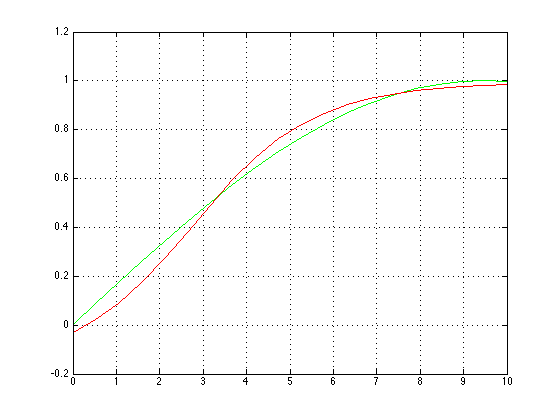
\includegraphics[width=300px]{img/rezultatas.png}
      \caption{Aproksimavimo rezultatas. Žalia linija žymi norimą išėjimą, Raudona linija žymi modelio išėjimą.}
      \label{fig:aproksimavimo_rezultatas}
    \end{figure}

    \section{Išvados}

    Laboratorinio darbo metu buvo sukurtas daugiasluoksnis (dviejų sluoksnių) perceptronų tinklas, nenaudojant MATLAB specializuotų funkcijų. Jis buvo apmokytas pasirinktos kreivės (sudarytai daugiau iš 20 atskaitų) aproksimuoti. Tinklo apmokymui buvo pritaikytas Backpropagation algoritmas. Aktyvavimo funkcijas neuronų tinkle pirmam sluoksnyje buvo pasirinktos eksponentinės funkcijas visuose perceptronuose. Paskutinio sluoksnio perceptrono aktyvavimo funkcija pasirinkta linijinė. Kreivė buvo sukurta, pritaikius šeštadalį sinuso kreivės.

\end{document}